%%%%%%%%%%%%%%%%%%%%%%%%%%%%%%%%%%%%%%%%%%%%%%%%%%%%%%%%%%%%%%%%%%%%%%%%%%%%%%%
\chapter{Elasticidade}
\label{Chap:ExpElasticidade}
%%%%%%%%%%%%%%%%%%%%%%%%%%%%%%%%%%%%%%%%%%%%%%%%%%%%%%%%%%%%%%%%%%%%%%%%%%%%%%%

\begin{fullwidth}\it
	Realizaremos um experimento visando mostrar o comportamento não-linear de um corpo que sofre uma deformação. Verificaremos através dos dados que a deformação segue uma forma característica conhecida como \emph{curva de histerese}. Veremos que as deformações com dependência linear na força aplicada se restringem a condições muito específicas. Utilizaremos os seguintes conceitos/técnicas de análise de dados: medidas, algarismos significativos, gráficos, e erros de escala e propagados.
\end{fullwidth}

%%%%%%%%%%%%%%%%%%%%%%%%%%%%%%%%%%%%%%%%%%%%%%%%%%%%%%%%%%%%%%%%%%%%%%%%%%%%%%%
\section{Elasticidade}
%%%%%%%%%%%%%%%%%%%%%%%%%%%%%%%%%%%%%%%%%%%%%%%%%%%%%%%%%%%%%%%%%%%%%%%%%%%%%%%

\begin{marginfigure}[7cm]
	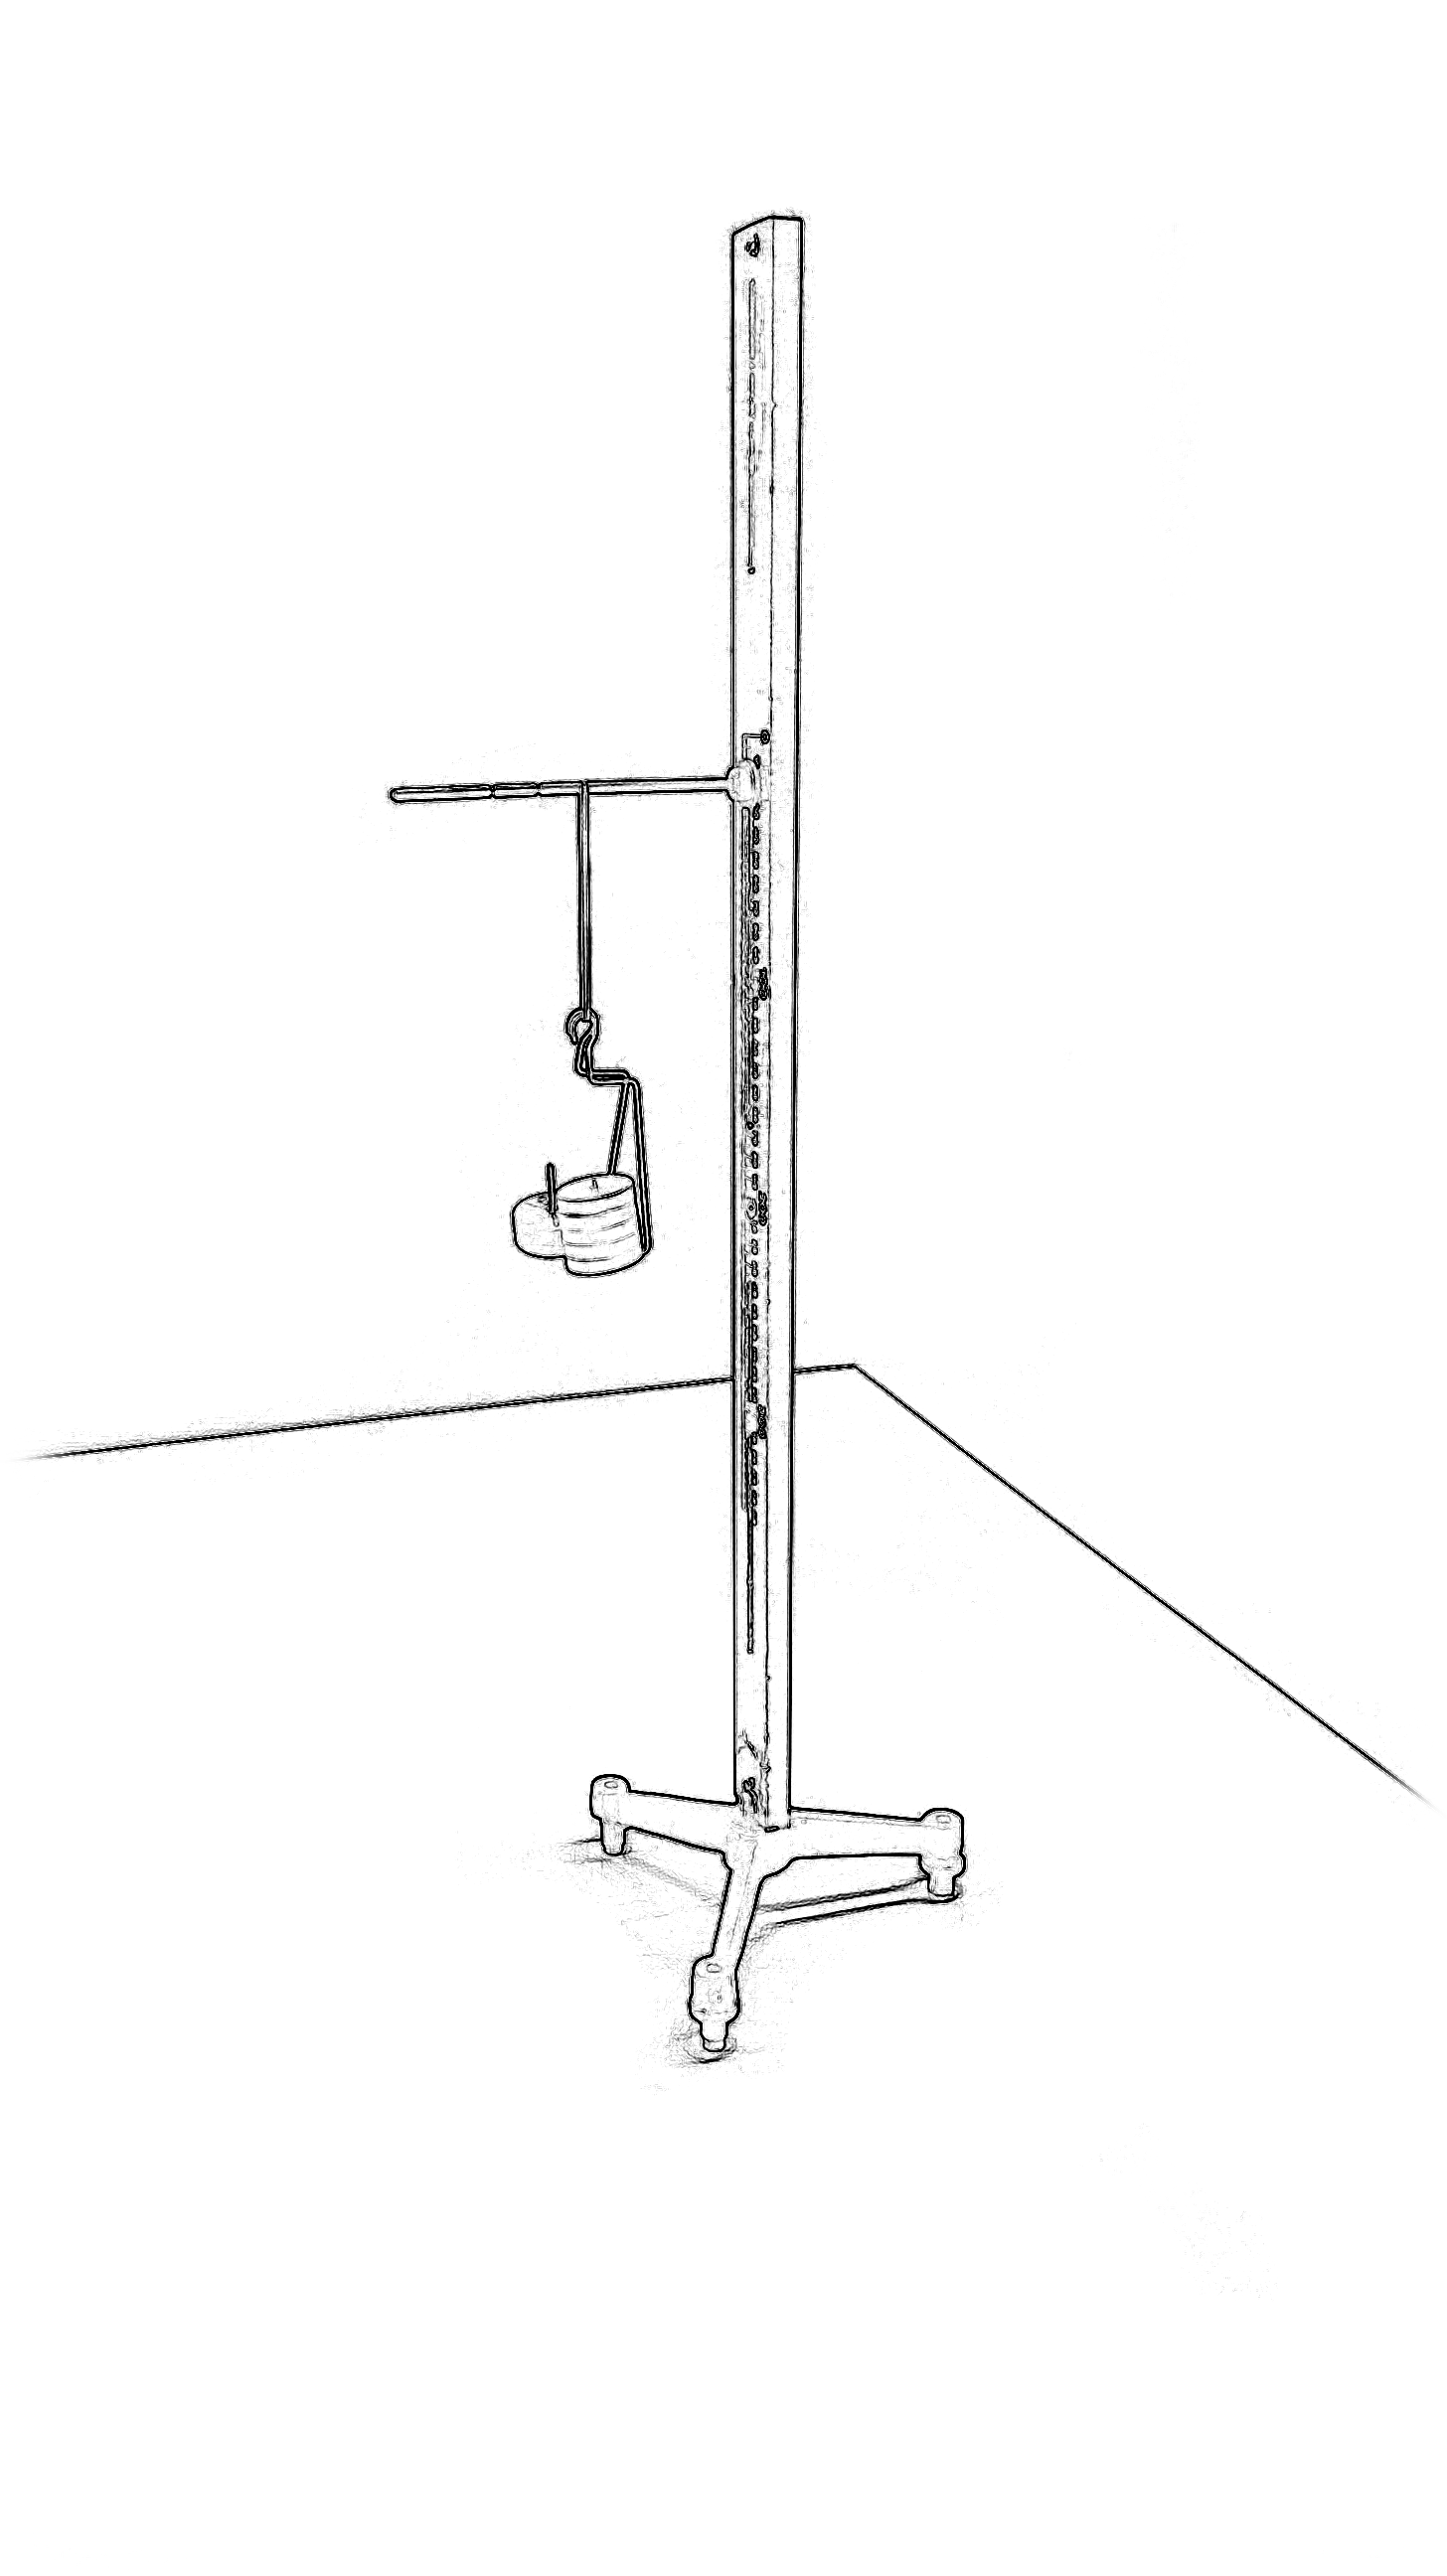
\includegraphics[width=\textwidth]{Ilustrations/Elasticidade.png}
	\caption{Ao submetermos um elástico a uma força variável, verificando a distensão registrada em função da força, obtemos uma \emph{curva de histerese}.}
\end{marginfigure}

Verificamos através da Lei de Hooke que a deformação de objetos em resposta a uma força aplicada é proporcional à intensidade da força:
\begin{equation}
	\Delta x = \frac{F}{k}.
\end{equation}

\noindent{}Sabemos, no entanto, que um objeto sujeito a uma força muito grande pode apresentar uma deformação permanente, ou mesmo se quebrar. Além disso, no caso mais geral, a deformação pode ser \emph{não-linear}.

Mesmo para uma mola, caso clássico em que se aplica a Lei de Hooke, a deformação será não-linear se a distensão da mola for muito grande. Por isso se faz a restrição de que \emph{a distensão da mola deve ser pequena}. Podemos entender melhor essa restrição chamando a força exercida pela mola de $f(x)$, onde $x$ representa a distensão da mola, e fazendo uma expansão de $f(x)$ em uma \emph{série de Taylor}. Esse tipo de expansão nos que diz que uma função $g(x)$ pode ser aproximada em torno de um ponto $x=a$ qualquer como
\begin{align}
	g(x) &= \sum_{n=1}^\infty \left[\frac{d^n}{dx^n}\frac{g(x)}{n!}\right]_{\mathrlap{x=a}}\cdot (x-a)^n \\
	&= \frac{g(a)}{0!} + \frac{g'(a)}{1!}(x - a) + \frac{g''(a)}{2!}(x-a)^2 + \frac{g'''(a)}{3!}(x-a)^3 + \dots \\
	&= g(a) + g'(a)(x-a) + \frac{g''(a)}{2}(x-a)^2 + \frac{g'''(a)}{6}(x-a)^3 + \dots,
\end{align}
%
onde $g'(a)$, $g''(a)$, $g'''(a)$, etc. são as derivadas da função $g(x)$ calculadas no ponto $a$.

Assim, podemos expandir a função $f(x)$ em torno de zero (considerando que esta é a posição de equilíbrio) como
\begin{equation}
	f(x) = f(0) + f'(0) (x-0) + \frac{f''(0)}{2}(x-0)^2 + \dots.
\end{equation}
%
No entanto, $f(0)$ é a força na posição de equilíbrio, ou seja, zero. Além disso, se $x$ é muito pequeno, temos que $x^2$ é menor ainda e por isso podemos desprezar todos os termos de ordem 2 (termos quadráticos) ou maior. Obtemos então:
\begin{equation}
	f(x) = f'(0)x,
\end{equation}
%
e se fizermos $k \equiv f'(0)$,
\begin{equation}
	f(x) = kx.
\end{equation}
%
Portanto, quando falamos em pequenas distensões, \emph{estamos restringindo os valores de termos de ordens quadrática ou superiores a valores muito menores que o termo de ordem linear}. Respeitada essa condição, o que poder ser feito através da escolha de uma distensão máxima adequada --- isto é, que ela seja suficientemente pequena para que os termos de ordem superior a 2 sejam desprezíveis ---, podemos tratar as deformações de um objeto como sendo lineares.

%%%%%%%%%%%%%%%%%%%%%%%%%%%%%%%%%%%%%
\subsection{Elasticidade e Histerese}
%%%%%%%%%%%%%%%%%%%%%%%%%%%%%%%%%%%%%

\begin{marginfigure}
	\centering
	\begin{tikzpicture}[scale=0.3, >=Stealth]
		\draw[very thin, ->] (-5,-4) -- +(10,0);
		\draw[very thin, ->] (-5,-4) -- +(0,8);
		\clip (-4,-4) rectangle (4,4);
		\draw[thick] (-5,-3) -- (-4,-3) to [controls={+(3,0) and +(-3,0)}] (2,3) -- (5,3);
		\draw[thick] (5,3) -- (4,3) to [controls={+(-3,0) and +(3,0)}] (-2,-3) -- (-5,-3);
	\end{tikzpicture}
	\caption{Gráfico típico de um fenômeno de histerese.}
	\label{Fig:Histerese}
\end{marginfigure}

Uma característica que também pode ser observada no caso de uma deformação não-linear é a \emph{histerese}. Temos na Figura~\ref{Fig:Histerese} uma típica figura de histerese: quando efetuamos um aumento gradual da variável independente, ocorre um aumento não-linear da variável dependente. Quando passamos a fazer uma diminuição da variável independente, existe uma diminuição correspondente da variável dependente, porém os valores não coincidem com aqueles do processo de aumento. Vários sistemas físicos têm esse tipo de comportamento: deformações de materiais, magnetização de imãs, campos elétricos em alguns materiais, etc.

Na Figura~\ref{Fig:HistereseElast} temos um gráfico da tensão em função deformação para um elástico de borracha. As linhas representam o processo de aumento e diminuição progressiva da tensão exercida sobre o elástico. Vemos que as duas curvas não coincidem. A explicação para este comportamento pode ser dada ao analisarmos o processo de um ponto de vista de energia: em uma mola, quando a esticamos, armazenamos energia potencial elástica. Já para um elástico de borracha, quando o esticamos, além de armazenarmos energia potencial elástica, também é possível notar um \emph{aumento da temperatura do elástico}, o que ocasiona uma perda de calor para o ambiente. Ao relaxarmos a distensão, é necessária a absorção de calor do meio. Como esse processo é demorado, se relaxarmos o elástico rapidamente, percebemos que ele não volta ao tamanho original. Após algum tempo, no entanto, a absorção de calor ocorre e o restaura ao tamanho inicial.

\begin{figure*}[!h]\forcerectofloat
	\centering
	\begin{tikzpicture}[gnuplot]
%% generated with GNUPLOT 5.0p0 (Lua 5.3; terminal rev. 99, script rev. 100)
%% 2015-07-06T11:33:50 BRT
\path (0.000,0.000) rectangle (14.000,9.000);
\gpcolor{color=gp lt color border}
\gpsetlinetype{gp lt border}
\gpsetdashtype{gp dt solid}
\gpsetlinewidth{1.00}
\draw[gp path] (1.136,1.268)--(1.316,1.268);
\draw[gp path] (13.447,1.268)--(13.267,1.268);
\node[gp node right] at (0.952,1.268) {$15$};
\draw[gp path] (1.136,2.684)--(1.316,2.684);
\draw[gp path] (13.447,2.684)--(13.267,2.684);
\node[gp node right] at (0.952,2.684) {$20$};
\draw[gp path] (1.136,4.100)--(1.316,4.100);
\draw[gp path] (13.447,4.100)--(13.267,4.100);
\node[gp node right] at (0.952,4.100) {$25$};
\draw[gp path] (1.136,5.516)--(1.316,5.516);
\draw[gp path] (13.447,5.516)--(13.267,5.516);
\node[gp node right] at (0.952,5.516) {$30$};
\draw[gp path] (1.136,6.932)--(1.316,6.932);
\draw[gp path] (13.447,6.932)--(13.267,6.932);
\node[gp node right] at (0.952,6.932) {$35$};
\draw[gp path] (1.136,8.348)--(1.316,8.348);
\draw[gp path] (13.447,8.348)--(13.267,8.348);
\node[gp node right] at (0.952,8.348) {$40$};
\draw[gp path] (1.649,0.985)--(1.649,1.165);
\draw[gp path] (1.649,8.631)--(1.649,8.451);
\node[gp node center] at (1.649,0.677) {$0$};
\draw[gp path] (3.701,0.985)--(3.701,1.165);
\draw[gp path] (3.701,8.631)--(3.701,8.451);
\node[gp node center] at (3.701,0.677) {$200$};
\draw[gp path] (5.753,0.985)--(5.753,1.165);
\draw[gp path] (5.753,8.631)--(5.753,8.451);
\node[gp node center] at (5.753,0.677) {$400$};
\draw[gp path] (7.804,0.985)--(7.804,1.165);
\draw[gp path] (7.804,8.631)--(7.804,8.451);
\node[gp node center] at (7.804,0.677) {$600$};
\draw[gp path] (9.856,0.985)--(9.856,1.165);
\draw[gp path] (9.856,8.631)--(9.856,8.451);
\node[gp node center] at (9.856,0.677) {$800$};
\draw[gp path] (11.908,0.985)--(11.908,1.165);
\draw[gp path] (11.908,8.631)--(11.908,8.451);
\node[gp node center] at (11.908,0.677) {$1000$};
\draw[gp path] (1.136,8.631)--(1.136,0.985)--(13.447,0.985)--(13.447,8.631)--cycle;
\node[gp node center,rotate=-270] at (0.246,4.808) {$L$~(cm)};
\node[gp node center] at (7.291,0.215) {$m$~(g)};
\node[gp node left] at (2.604,8.297) {carga};
\gpcolor{rgb color={0.000,0.000,0.000}}
\gpsetlinewidth{2.00}
\gpsetpointsize{4.00}
\gppoint{gp mark 9}{(2.235,1.835)}
\gppoint{gp mark 9}{(2.747,1.948)}
\gppoint{gp mark 9}{(3.259,2.004)}
\gppoint{gp mark 9}{(3.771,2.146)}
\gppoint{gp mark 9}{(4.273,2.259)}
\gppoint{gp mark 9}{(4.870,2.373)}
\gppoint{gp mark 9}{(5.374,2.571)}
\gppoint{gp mark 9}{(5.887,2.741)}
\gppoint{gp mark 9}{(6.399,2.967)}
\gppoint{gp mark 9}{(6.902,3.222)}
\gppoint{gp mark 9}{(7.481,3.647)}
\gppoint{gp mark 9}{(7.990,4.015)}
\gppoint{gp mark 9}{(8.504,4.553)}
\gppoint{gp mark 9}{(9.014,4.950)}
\gppoint{gp mark 9}{(9.527,5.374)}
\gppoint{gp mark 9}{(10.114,5.941)}
\gppoint{gp mark 9}{(10.627,6.252)}
\gppoint{gp mark 9}{(11.140,6.649)}
\gppoint{gp mark 9}{(11.653,7.130)}
\gppoint{gp mark 9}{(12.160,7.272)}
\gppoint{gp mark 9}{(1.962,8.297)}
\draw[gp path] (2.235,1.838)--(2.335,1.857)--(2.435,1.877)--(2.536,1.896)--(2.636,1.914)%
  --(2.736,1.932)--(2.836,1.949)--(2.937,1.966)--(3.037,1.983)--(3.137,2.001)--(3.237,2.019)%
  --(3.338,2.039)--(3.438,2.061)--(3.538,2.083)--(3.638,2.107)--(3.739,2.130)--(3.839,2.153)%
  --(3.939,2.176)--(4.039,2.198)--(4.140,2.221)--(4.240,2.243)--(4.340,2.265)--(4.440,2.286)%
  --(4.541,2.309)--(4.641,2.332)--(4.741,2.357)--(4.841,2.384)--(4.942,2.413)--(5.042,2.444)%
  --(5.142,2.477)--(5.242,2.510)--(5.343,2.545)--(5.443,2.580)--(5.543,2.616)--(5.643,2.652)%
  --(5.744,2.689)--(5.844,2.727)--(5.944,2.766)--(6.044,2.807)--(6.145,2.849)--(6.245,2.893)%
  --(6.345,2.939)--(6.445,2.986)--(6.546,3.036)--(6.646,3.088)--(6.746,3.143)--(6.846,3.201)%
  --(6.947,3.262)--(7.047,3.326)--(7.147,3.393)--(7.247,3.463)--(7.348,3.535)--(7.448,3.609)%
  --(7.548,3.685)--(7.648,3.763)--(7.749,3.843)--(7.849,3.925)--(7.949,4.011)--(8.049,4.099)%
  --(8.150,4.190)--(8.250,4.283)--(8.350,4.376)--(8.450,4.469)--(8.551,4.559)--(8.651,4.648)%
  --(8.751,4.734)--(8.852,4.820)--(8.952,4.905)--(9.052,4.989)--(9.152,5.074)--(9.253,5.159)%
  --(9.353,5.245)--(9.453,5.332)--(9.553,5.419)--(9.654,5.507)--(9.754,5.595)--(9.854,5.683)%
  --(9.954,5.769)--(10.055,5.852)--(10.155,5.932)--(10.255,6.008)--(10.355,6.082)--(10.456,6.156)%
  --(10.556,6.229)--(10.656,6.303)--(10.756,6.378)--(10.857,6.455)--(10.957,6.534)--(11.057,6.613)%
  --(11.157,6.693)--(11.258,6.774)--(11.358,6.853)--(11.458,6.929)--(11.558,7.000)--(11.659,7.065)%
  --(11.759,7.122)--(11.859,7.173)--(11.959,7.220)--(12.060,7.263)--(12.160,7.305);
\gpcolor{color=gp lt color border}
\node[gp node left] at (2.604,7.989) {descarga};
\gpcolor{rgb color={0.000,0.000,0.000}}
\gppoint{gp mark 11}{(12.160,7.272)}
\gppoint{gp mark 11}{(11.653,7.328)}
\gppoint{gp mark 11}{(11.140,7.272)}
\gppoint{gp mark 11}{(10.627,7.215)}
\gppoint{gp mark 11}{(10.114,7.158)}
\gppoint{gp mark 11}{(9.527,7.045)}
\gppoint{gp mark 11}{(9.014,6.960)}
\gppoint{gp mark 11}{(8.504,6.819)}
\gppoint{gp mark 11}{(7.990,6.677)}
\gppoint{gp mark 11}{(7.481,6.450)}
\gppoint{gp mark 11}{(6.902,6.139)}
\gppoint{gp mark 11}{(6.399,5.799)}
\gppoint{gp mark 11}{(5.887,5.374)}
\gppoint{gp mark 11}{(5.374,4.950)}
\gppoint{gp mark 11}{(4.870,4.468)}
\gppoint{gp mark 11}{(4.273,3.789)}
\gppoint{gp mark 11}{(3.771,3.449)}
\gppoint{gp mark 11}{(3.259,3.109)}
\gppoint{gp mark 11}{(2.747,2.712)}
\gppoint{gp mark 11}{(2.235,2.401)}
\gppoint{gp mark 11}{(1.962,7.989)}
\draw[gp path] (2.235,2.394)--(2.335,2.459)--(2.435,2.524)--(2.536,2.589)--(2.636,2.655)%
  --(2.736,2.722)--(2.836,2.791)--(2.937,2.861)--(3.037,2.931)--(3.137,3.002)--(3.237,3.072)%
  --(3.338,3.141)--(3.438,3.210)--(3.538,3.279)--(3.638,3.348)--(3.739,3.418)--(3.839,3.489)%
  --(3.939,3.563)--(4.039,3.640)--(4.140,3.721)--(4.240,3.807)--(4.340,3.899)--(4.440,3.997)%
  --(4.541,4.098)--(4.641,4.202)--(4.741,4.307)--(4.841,4.412)--(4.942,4.516)--(5.042,4.618)%
  --(5.142,4.718)--(5.242,4.815)--(5.343,4.910)--(5.443,5.002)--(5.543,5.092)--(5.643,5.180)%
  --(5.744,5.266)--(5.844,5.351)--(5.944,5.435)--(6.044,5.517)--(6.145,5.598)--(6.245,5.677)%
  --(6.345,5.754)--(6.445,5.828)--(6.546,5.901)--(6.646,5.970)--(6.746,6.038)--(6.846,6.102)%
  --(6.947,6.164)--(7.047,6.224)--(7.147,6.281)--(7.247,6.335)--(7.348,6.388)--(7.448,6.438)%
  --(7.548,6.485)--(7.648,6.531)--(7.749,6.574)--(7.849,6.615)--(7.949,6.653)--(8.049,6.689)%
  --(8.150,6.723)--(8.250,6.754)--(8.350,6.784)--(8.450,6.813)--(8.551,6.840)--(8.651,6.867)%
  --(8.751,6.892)--(8.852,6.916)--(8.952,6.940)--(9.052,6.962)--(9.152,6.982)--(9.253,7.002)%
  --(9.353,7.021)--(9.453,7.040)--(9.553,7.058)--(9.654,7.076)--(9.754,7.093)--(9.854,7.111)%
  --(9.954,7.127)--(10.055,7.143)--(10.155,7.159)--(10.255,7.173)--(10.355,7.186)--(10.456,7.199)%
  --(10.556,7.212)--(10.656,7.224)--(10.756,7.236)--(10.857,7.248)--(10.957,7.259)--(11.057,7.270)%
  --(11.157,7.280)--(11.258,7.288)--(11.358,7.296)--(11.458,7.302)--(11.558,7.306)--(11.659,7.307)%
  --(11.759,7.306)--(11.859,7.303)--(11.959,7.297)--(12.060,7.291)--(12.160,7.284);
\gpcolor{color=gp lt color border}
\gpsetlinewidth{1.00}
\draw[gp path] (1.136,8.631)--(1.136,0.985)--(13.447,0.985)--(13.447,8.631)--cycle;
%% coordinates of the plot area
\gpdefrectangularnode{gp plot 1}{\pgfpoint{1.136cm}{0.985cm}}{\pgfpoint{13.447cm}{8.631cm}}
\end{tikzpicture}
%% gnuplot variables

	\caption{Gráfico de histerese para o processo de carregamento e descarregamento de um elástico. Note que o último ponto do processo de carga e o primeiro do processo de descarga coincidem. As linhas foram ajustadas utilizando uma spline de aproximação cúbica de Hermite.}
	\label{Fig:HistereseElast}
\end{figure*}

Esse fenômeno pode ser entendido analisando a estrutura da borracha: ela é constituída de moléculas de polímeros de tamanhos diferentes, constituindo um emaranhado de fibras. Devido à agitação térmica das moléculas ---~agitação característica dos corpos a nível molecular associada à temperatura~--- as moléculas sofrem colisões laterais sucessivas, encurtando-se. Quando esticamos o elástico, as moléculas alinham-se, colidindo lateralmente contra as menores, transferindo energia cinética e aumentando a temperatura. Se o processo de esticamento demora tempo suficente para que o calor seja transferido para o meio ---~através de colisões das moléculas mais próximas da superfície com as moléculas do ar, por exemplo, transferindo energia cinética para fora da borracha~---, ao relaxarmos o elástico, não há energia suficiente nas moléculas menores para que elas colidam com as maiores e façam com que elas se contraiam totalmente. Portanto, há uma deformação residual no elástico.

%%%%%%%%%%%%%%%%%%%%%%%%%%%%%%%%%%%%%%%%%%%%%%%%%%%%%%%%%%%%%%%%%%%%%%%%%%%%%%%
\section{Experimento}
%%%%%%%%%%%%%%%%%%%%%%%%%%%%%%%%%%%%%%%%%%%%%%%%%%%%%%%%%%%%%%%%%%%%%%%%%%%%%%%

Realizaremos um experimento para verificar a curva de histerese do comprimento de um elástico de borracha: vamos pendurar o elástico em uma haste horizontal e na extremidade oposta vamos pendurar um gancho ao qual adicionaremos anilhas. Devido as propriedades da borracha, verificaremos um comportamento diverso ao de uma mola.

%%%%%%%%%%%%%%%%%%%%%%
\subsection{Objetivos}
\label{Sec:ObjetivosElasticidade}
%%%%%%%%%%%%%%%%%%%%%%

\begin{enumerate}
%	\item Verificar o melhor valor para a medida da massa de um conjunto de anilhas através do valor médio;
%	\item Calcular o desvio padrão dos valores da massa e o valor do desvio padrão da média;
	\item Realizar as medidas de deformação de um elástico verificando a curva de histerese resultante;
	\item Verificar a dissipação de energia envolvida em processos que não são elásticos. 
\end{enumerate}

%%%%%%%%%%%%%%%%%%%%%%%%%%%%%%%%%%%%%%%%%%%%%%%%%%%%%%%%%%%%%%%%%%%%%%%%%%%%%%%
\section{Material Necessário}
%%%%%%%%%%%%%%%%%%%%%%%%%%%%%%%%%%%%%%%%%%%%%%%%%%%%%%%%%%%%%%%%%%%%%%%%%%%%%%%

\begin{itemize}
	\item 20 anilhas metálicas e ganchos adequados para suportá-las;
	\item Suporte vertical com haste horizontal;
	\item Elástico de borracha;
	\item Régua;
	\item Balança de braços.
\end{itemize}

%%%%%%%%%%%%%%%%%%%%%%%%%%%%%%%%%%%%%%%%%%%%%%%%%%%%%%%%%%%%%%%%%%%%%%%%%%%%%%%
\section{Procedimento Experimental}
%%%%%%%%%%%%%%%%%%%%%%%%%%%%%%%%%%%%%%%%%%%%%%%%%%%%%%%%%%%%%%%%%%%%%%%%%%%%%%%

\begin{enumerate}
    \item Enumere as anilhas a lápis, pois posteriormente elas deverão ser retiradas na ordem inversa em que foram colocadas;
	\item Verifique a massa $m_a$ de cada uma das anilhas e anote na Tabela~\ref{tab:ComprimentoElastico};
	\item Verifique a massa $m_g$ dos ganchos e anote na Tabela~\ref{tab:ComprimentoElastico};
	\item Na haste horizontal do suporte pendure um elástico de borracha e na sua extremidade livre pendure um gancho com uma anilha;
	\item Meça o comprimento $\ell$ do elástico e o anote, juntamente com a massa total $m_t$ sustentada pelo elástico, nas colunas correspondentes ao processo de ``carga'' da Tabela~\ref{tab:ComprimentoElastico};
	\item Adicione mais uma anilha e verifique o novo comprimento, anotando os dados para $\ell$ e $m_t$ na Tabela~\ref{tab:ComprimentoElastico};
	\item Repita o item acima até que todas as anilhas tenham sido penduradas. Utilize ganchos adicionais quando necessário. Não esqueça de somar a massa do gancho;
	\item Anote os últimos os valores\footnote{Atenção: se houver demora para iniciar o processo de descarga, pode ser necessário realizar uma nova medida de comprimento, pois é comum que o elástico continue cedendo lentamente ao peso suspenso.} de comprimento e massa do processo de ``carregamento'' também nas colunas relativas ao processo de ``descarregamento'' Tabela~\ref{tab:ComprimentoElastico};
	\item Retire as anilhas suspensas pelo elástico uma a uma, realizando o processo inverso ao ``carregamento'', anotando os valores de massa e comprimento correspondentes.
\end{enumerate}

%%%%%%%%%%%%%%%%%%%%%%%%%%%%%%%%%%%%%%%%%%%%%%%%%%%%%%%%%%%%%%%%%%%%%%%%%%%%%%%
%%%%%%%%%%%%%%%%%%%%%%%%%%%%%%%%%%%%%%%%%%%%%%%%%%%%%%%%%%%%%%%%%%%%%%%%%%%%%%%
%%%%%%%%%%%%%%%%%%%%%%%%%%%%%%%%%%%%%%%%%%%%%%%%%%%%%%%%%%%%%%%%%%%%%%%%%%%%%%%
%%%%%%%%%%%%%%%%%%%%%%%%%%%%%%%%%%%%%%%%%%%%%%%%%%%%%%%%%%%%%%%%%%%%%%%%%%%%%%%
\cleardoublepage

\noindent{}{\huge\textit{Elasticidade}}

\vspace{15mm}

\begin{fullwidth}
\noindent{}\makebox[0.6\linewidth]{Turma:\enspace\hrulefill}\makebox[0.4\textwidth]{  Data:\enspace\hrulefill}
\vspace{5mm}

\noindent{}\makebox[0.6\linewidth]{Aluno(a):\enspace\hrulefill}\makebox[0.4\textwidth]{  Matrícula:\enspace\hrulefill}

\noindent{}\makebox[0.6\linewidth]{Aluno(a):\enspace\hrulefill}\makebox[0.4\textwidth]{  Matrícula:\enspace\hrulefill}

\noindent{}\makebox[0.6\linewidth]{Aluno(a):\enspace\hrulefill}\makebox[0.4\textwidth]{  Matrícula:\enspace\hrulefill}

\noindent{}\makebox[0.6\linewidth]{Aluno(a):\enspace\hrulefill}\makebox[0.4\textwidth]{  Matrícula:\enspace\hrulefill}

\noindent{}\makebox[0.6\linewidth]{Aluno(a):\enspace\hrulefill}\makebox[0.4\textwidth]{  Matrícula:\enspace\hrulefill}
\end{fullwidth}

\vspace{5mm}

%%%%%%%%%%%%%%%%%%%%%%%%%%%%%%%%%%%%%%%%%%%%%%%%%%%%%%%%%%%%%%%%%%%%%%%%%%%%%%%
\section{Questionário}
%%%%%%%%%%%%%%%%%%%%%%%%%%%%%%%%%%%%%%%%%%%%%%%%%%%%%%%%%%%%%%%%%%%%%%%%%%%%%%%

\begin{question}[type={exam}]{1}
Liste os instrumentos de medida utilizados. Descreva o tipo do equipamento, sua resolução, e seu erro de escala.
\end{question}

\begin{question}[type={exam}]{2}
Preencha as tabelas com o número adequado de algarismos significativos, unidades, e erros de escala apropriados. 
\end{question}

\begin{question}[type={exam}]{3}
Elabore um gráfico de $\ell \times m$ ---~onde $\ell$ é o comprimento do elástico e $m$ é a massa total correspondente ao conjunto de anilhas e ganchos que o elástico sustenta~---. Ambos os conjuntos de dados (``carregamento'' e ``descarregamento'' na Tabela~\ref{tab:ComprimentoElastico}) devem estar contidos no mesmo gráfico, sendo que os pontos de cada conjunto de dados devem estar claramente diferenciados.
\end{question}

\begin{question}[type={exam}]{2}
\begin{enumerate}[label=\roman*.]
\item Calcule a diferença entre os comprimentos do elástico quando ele suporta somente uma anilha no processo de carga e no processo de descarga (a diferença entre a primeira medida realizada no carregamento e a última no descarregamento).
\item Através de tal valor, calcule a diferença de energia potencial gravitacional entre as duas posições.
\item O que acontece com a energia potencial perdida?\footnote{\emph{A energia não fica armazenada como energia potencial elástica!}}
\end{enumerate}
\end{question}

\begin{question}[type={exam}]{2}
Considerando os objetivos do experimento, listados na Seção~\ref{Sec:ObjetivosElasticidade}, e os resultados obtidos nas questões anteriores, discuta quais objetivos foram atingidos com sucesso, justificando suas conclusões. Se algum objetivo não foi atingido, discuta quais são os possíveis motivos do insucesso e que providências podem ser tomadas para que eles sejam alcançados.
\end{question}
\vfill

%%%%%%%%%%%%%%%%%%%%%%%%%%%%%%%%%%%%%%%%%%%%%%%%%%%%%%%%%%%%%%%%%%%%%%%%%%%%%%%
\pagebreak
\section{Tabelas}
%%%%%%%%%%%%%%%%%%%%%%%%%%%%%%%%%%%%%%%%%%%%%%%%%%%%%%%%%%%%%%%%%%%%%%%%%%%%%%%

\begin{table*}
	\begin{center}
		\begin{tabular}{llp{25mm}lp{25mm}p{25mm}lp{25mm}p{25mm}l}
		\toprule
		& N\textordmasculine & \textbf{$m_g$} & \\
		\cmidrule{2-3}
		& 1 & \cellcolor[gray]{0.89} \\
		& 2 & \cellcolor[gray]{0.95} \\
		& 3 & \cellcolor[gray]{0.89} \\
		& 4 & \cellcolor[gray]{0.95} \\
		\cmidrule{2-3}
\\
		& & & & \multicolumn{2}{c}{\textbf{Carregamento}} & & \multicolumn{2}{c}{\textbf{Descarregamento}} \\
		\cmidrule{5-6} \cmidrule{8-9}
		& N\textordmasculine & \textbf{$m_a$} & & $\ell$ & \multicolumn{1}{c}{$m_t$} & & $\ell$ & \multicolumn{1}{c}{$m_t$} \\
		\cmidrule{2-3} \cmidrule{5-6} \cmidrule{8-9}
		&  1 & \cellcolor[gray]{0.89} & & \cellcolor[gray]{0.89} & \cellcolor[gray]{0.92} & & \cellcolor[gray]{0.89} & \cellcolor[gray]{0.92} & \\
		&  2 & \cellcolor[gray]{0.95} & & \cellcolor[gray]{0.95} & \cellcolor[gray]{0.97} & & \cellcolor[gray]{0.95} & \cellcolor[gray]{0.97} & \\
		&  3 & \cellcolor[gray]{0.89} & & \cellcolor[gray]{0.89} & \cellcolor[gray]{0.92} & & \cellcolor[gray]{0.89} & \cellcolor[gray]{0.92} & \\
		&  4 & \cellcolor[gray]{0.95} & & \cellcolor[gray]{0.95} & \cellcolor[gray]{0.97} & & \cellcolor[gray]{0.95} & \cellcolor[gray]{0.97} & \\
		&  5 & \cellcolor[gray]{0.89} & & \cellcolor[gray]{0.89} & \cellcolor[gray]{0.92} & & \cellcolor[gray]{0.89} & \cellcolor[gray]{0.92} & \\
		&  6 & \cellcolor[gray]{0.95} & & \cellcolor[gray]{0.95} & \cellcolor[gray]{0.97} & & \cellcolor[gray]{0.95} & \cellcolor[gray]{0.97} & \\
		&  7 & \cellcolor[gray]{0.89} & & \cellcolor[gray]{0.89} & \cellcolor[gray]{0.92} & & \cellcolor[gray]{0.89} & \cellcolor[gray]{0.92} & \\
		&  8 & \cellcolor[gray]{0.95} & & \cellcolor[gray]{0.95} & \cellcolor[gray]{0.97} & & \cellcolor[gray]{0.95} & \cellcolor[gray]{0.97} & \\
		&  9 & \cellcolor[gray]{0.89} & & \cellcolor[gray]{0.89} & \cellcolor[gray]{0.92} & & \cellcolor[gray]{0.89} & \cellcolor[gray]{0.92} & \\
		& 10 & \cellcolor[gray]{0.95} & & \cellcolor[gray]{0.95} & \cellcolor[gray]{0.97} & & \cellcolor[gray]{0.95} & \cellcolor[gray]{0.97} & \\
		& 11 & \cellcolor[gray]{0.89} & & \cellcolor[gray]{0.89} & \cellcolor[gray]{0.92} & & \cellcolor[gray]{0.89} & \cellcolor[gray]{0.92} & \\
		& 12 & \cellcolor[gray]{0.95} & & \cellcolor[gray]{0.95} & \cellcolor[gray]{0.97} & & \cellcolor[gray]{0.95} & \cellcolor[gray]{0.97} & \\
		& 13 & \cellcolor[gray]{0.89} & & \cellcolor[gray]{0.89} & \cellcolor[gray]{0.92} & & \cellcolor[gray]{0.89} & \cellcolor[gray]{0.92} & \\
		& 14 & \cellcolor[gray]{0.95} & & \cellcolor[gray]{0.95} & \cellcolor[gray]{0.97} & & \cellcolor[gray]{0.95} & \cellcolor[gray]{0.97} & \\
		& 15 & \cellcolor[gray]{0.89} & & \cellcolor[gray]{0.89} & \cellcolor[gray]{0.92} & & \cellcolor[gray]{0.89} & \cellcolor[gray]{0.92} & \\
		& 16 & \cellcolor[gray]{0.95} & & \cellcolor[gray]{0.95} & \cellcolor[gray]{0.97} & & \cellcolor[gray]{0.95} & \cellcolor[gray]{0.97} & \\
		& 17 & \cellcolor[gray]{0.89} & & \cellcolor[gray]{0.89} & \cellcolor[gray]{0.92} & & \cellcolor[gray]{0.89} & \cellcolor[gray]{0.92} & \\
		& 18 & \cellcolor[gray]{0.95} & & \cellcolor[gray]{0.95} & \cellcolor[gray]{0.97} & & \cellcolor[gray]{0.95} & \cellcolor[gray]{0.97} & \\
		& 19 & \cellcolor[gray]{0.89} & & \cellcolor[gray]{0.89} & \cellcolor[gray]{0.92} & & \cellcolor[gray]{0.89} & \cellcolor[gray]{0.92} & \\
		& 20 & \cellcolor[gray]{0.95} & & \cellcolor[gray]{0.95} & \cellcolor[gray]{0.97} & & \cellcolor[gray]{0.95} & \cellcolor[gray]{0.97} & \\
\bottomrule
		\end{tabular}
	\caption[][2mm]{Dados obtidos para o comprimento do elástico e a massa correspondente.}\label{tab:ComprimentoElastico}
	\end{center}
\end{table*}

